\section{Backend Testing}

The CFI-Care backend is covered by an automated test suite built on
\textbf{Jest v30.2.0} with \textbf{Supertest v7.2.2} for HTTP-layer assertions.
The suite comprises 34 test files organized into five categories: FHIR resource
service unit tests, HTTP route contract tests, service integration tests, utility
and middleware tests, and end-to-end workflow tests. All tests run inside a
Node.js environment; external dependencies (FHIR server, Redis, PostgreSQL) are
mocked in unit and route tests, and live instances are exercised only in
explicitly-named integration tests.

\subsection{Framework and Configuration}

Jest is configured in \texttt{jest.config.js} with the test environment set to
\texttt{node} and a global timeout of 10 seconds per test. Test discovery
targets both the source tree and the sibling \texttt{tests/} directory, matching
any file that ends in \texttt{.test.js} or \texttt{.spec.js}. After each suite
Jest generates three report artefacts: a JUnit XML file consumed by CI pipelines,
an HTML summary for human review, and per-format coverage reports (\texttt{lcov},
\texttt{clover}, JSON).

\subsubsection{Coverage Thresholds}
A global coverage gate of 70\% is enforced across all four metrics---branches,
functions, lines, and statements---so that Jest exits non-zero if coverage falls
below this floor:

\begin{center}\small
\begin{tabular}{lcc}
\hline
\textbf{Metric} & \textbf{Threshold} & \textbf{Scope} \\
\hline
Branches    & 70\% & global \\
Functions   & 70\% & global \\
Lines       & 70\% & global \\
Statements  & 70\% & global \\
\hline
\end{tabular}
\end{center}

\subsubsection{Test Scripts}
The \texttt{package.json} exposes dedicated npm scripts for each test category,
allowing selective or full execution:

\begin{itemize}
  \item \texttt{test} --- all suites except the live database probe (default CI target).
  \item \texttt{test:all} --- all suites including live Redis and Postgres checks.
  \item \texttt{test:coverage} --- full run with coverage collection and threshold enforcement.
  \item \texttt{test:unit} --- validation and middleware suites only.
  \item \texttt{test:integration} --- service integration and route contract suites.
  \item \texttt{test:e2e} --- end-to-end workflow suites only.
  \item \texttt{test:history-graph} --- all history-graph-related suites in isolation.
\end{itemize}

All scripts pass \texttt{--runInBand} to execute suites sequentially, preventing
race conditions on shared mock state, and \texttt{--forceExit} to terminate the
process after the last assertion.

\subsection{Test Suite Inventory}

Table~\ref{tab:backend-test-suites} lists every test file, its category, and its
primary focus area.

\begin{table}[H]
\centering
\caption{Backend Test Suite Inventory}
\label{tab:backend-test-suites}
\setlength{\tabcolsep}{4pt}
\begin{tabular}{|p{5.5cm}|p{2.2cm}|p{6cm}|}
\hline
\textbf{Test File} & \textbf{Category} & \textbf{Focus} \\
\hline
\multicolumn{3}{|l|}{\textit{FHIR Resource Service Unit Tests (20 files)}} \\ \hline
allergyIntoleranceService & Unit & Cache-first reads, create/update/delete, 404 and FHIR validation errors \\
appointmentService        & Unit & Appointment CRUD, slot conflict handling, FHIR bundle responses \\
deviceService             & Unit & Device read/write, cache invalidation, error propagation \\
diagnosticReportService   & Unit & Report fetch, patient-scoped bundles, create and update \\
documentReferenceService  & Unit & Document fetch, binary linking, validation errors \\
encounterService          & Unit & Encounter CRUD, \texttt{\$everything} bundle aggregation \\
eocService                & Unit & Episode-of-care lifecycle, create and query \\
healthcareServiceService  & Unit & Service directory queries, cache hits and misses \\
imagingStudyService       & Unit & Imaging resource CRUD, FHIR payload structure \\
immunizationService       & Unit & Immunization records, patient-scoped queries \\
locationService           & Unit & Location read/write, cache TTL behavior \\
medicationRequestService  & Unit & Medication CRUD, dispense status, error handling \\
observationService        & Unit & Vital-sign observations, bundle responses, 404 paths \\
organizationService       & Unit & Organization read/write, cache invalidation \\
practionerService         & Unit & Practitioner CRUD, JWKS identity binding \\
practitionerRoleService   & Unit & Role assignments, scoped queries \\
procedureService          & Unit & Procedure records, create/update/soft-delete \\
relatedPersonService      & Unit & Related-person relationships, patient linkage \\
scheduleService           & Unit & Schedule CRUD, time-slot alignment \\
slotService               & Unit & Slot availability, booking state transitions \\
\hline
\multicolumn{3}{|l|}{\textit{HTTP Route Contract Tests (4 files)}} \\ \hline
patientRoutes             & Route & CRUD, TOON export, related-data aggregation \\
encounterRoutes           & Route & Encounter fetch and \texttt{\$everything} retrieval \\
binaryRoutes              & Route & PDF fetch/create/delete, required-field validation \\
historyGraphRoutes        & Route & Graph init, head-node CRUD, node seeding \\
\hline
\multicolumn{3}{|l|}{\textit{Service Integration Tests (3 files)}} \\ \hline
patientService.integration      & Integration & Cache-first reads, FHIR fallbacks, \texttt{\$everything} \\
conditionService.integration    & Integration & Patient-scoped condition queries, create/update \\
historyGraphService.integration & Integration & Node and edge CRUD, branch state, cache interaction \\
\hline
\multicolumn{3}{|l|}{\textit{Utility and Middleware Tests (4 files)}} \\ \hline
cacheHelper               & Unit & get/set/delete semantics, TTL, error tolerance \\
patientValidation         & Unit & Joi schema enforcement on patient payloads \\
validateRequest           & Unit & Middleware pass/fail branch coverage \\
redis                     & Integration* & Live Redis CRUD, TTL expiry, data-type support \\
\hline
\multicolumn{3}{|l|}{\textit{Infrastructure Tests (1 file)}} \\ \hline
database                  & Integration* & Postgres connectivity, schema probing \\
\hline
\multicolumn{3}{|l|}{\textit{End-to-End Workflow Tests (2 files)}} \\ \hline
patient-workflow.e2e      & E2E & Patient management lifecycle \\
historyGraph-workflow.e2e & E2E & Graph lifecycle including branching and linker nodes \\
\hline
\multicolumn{3}{l}{\footnotesize * Requires a live backing service; excluded from the default CI target.}
\end{tabular}
\end{table}

\subsection{Mocking Strategy}

Consistent mocking conventions are established once in the Jest setup file and
reused across suites:

\begin{itemize}
  \item \textbf{FHIR API (axios):} \texttt{axios.create()} is replaced with a
        factory that returns a shared mock instance exposing \texttt{get},
        \texttt{post}, \texttt{put}, and \texttt{delete} spies. Each test
        configures return values with \texttt{mockResolvedValue} or
        \texttt{mockRejectedValue}, enabling both success and failure paths
        without network calls.
  \item \textbf{Redis (cacheHelper):} The \texttt{cacheHelper} middleware is
        mocked to expose \texttt{getFromCache}, \texttt{setInCache}, and
        \texttt{deleteFromCache} spies. Cache-hit tests pre-load
        \texttt{getFromCache} with a resolved value; cache-miss tests leave it
        returning \texttt{null}, forcing the code path through to the FHIR call.
  \item \textbf{PostgreSQL (pg):} The \texttt{pg} module is replaced with a
        mock \texttt{Pool} and \texttt{Client} whose \texttt{query} method is a
        spy defaulting to \texttt{\{ rows: [] \}}. The history graph service
        tests reconfigure \texttt{query} on a per-scenario basis to simulate
        node insertion, edge creation, and soft-delete responses.
  \item \textbf{Authentication middleware:} \texttt{requireApiAuth},
        \texttt{requirePatientContext}, and \texttt{validateScopes} are replaced
        with pass-through functions (\texttt{(req, res, next) => next()}) in all
        route and e2e tests, isolating HTTP contract verification from the
        auth layer.
\end{itemize}

\texttt{jest.clearAllMocks()} is called in every \texttt{beforeEach} block,
ensuring that call history and resolved values do not bleed between test cases.

\subsection{FHIR Resource Service Unit Tests}

The 20 FHIR resource service suites each follow an identical structural pattern
that exercises three behavioral axes: caching, FHIR API interaction, and error
propagation.

\subsubsection{Cache-First Read Path}
For every read operation (GET by ID, list by patient), the service first queries
Redis. If a valid entry is found, the data is returned immediately and the FHIR
call is skipped. Tests assert that \texttt{getFromCache} was called once and that
the FHIR spy was never invoked.

\subsubsection{Cache-Miss and Fallback}
When \texttt{getFromCache} returns \texttt{null}, the service calls the FHIR
server, stores the result via \texttt{setInCache}, and returns it to the caller.
Tests assert that both the FHIR spy and \texttt{setInCache} were called, and that
the response body matches the mocked FHIR payload.

\subsubsection{Write-Triggered Cache Invalidation}
Create, update, and delete operations call \texttt{deleteFromCache} for the
affected resource keys before returning. Tests verify that invalidation targets
the correct key namespaces (e.g., \texttt{patient:\{id\}} and
\texttt{encounters:patient:\{id\}}) so that the next read forces a fresh FHIR
query.

\subsubsection{Error Handling}
Each service suite includes negative-path cases:
\begin{itemize}
  \item \textbf{404 Not Found} --- FHIR returns an \texttt{OperationOutcome} with
        \texttt{issue[0].severity = error}; the service propagates a 404 to the
        caller.
  \item \textbf{422 Unprocessable} --- FHIR returns validation diagnostics; the
        service surfaces the \texttt{diagnostics} field.
  \item \textbf{Network failure} --- axios rejects with a connection error; the
        service re-throws so the route layer can return a 500.
\end{itemize}

\subsection{Service Integration Tests}

The three integration test files exercise complete service workflows using mocked
infrastructure (postgres, axios, and cache spies) but without an intermediary
route layer.

\begin{itemize}
  \item \textbf{patientService.integration} --- covers cache-first patient reads,
        FHIR fallbacks, patient creation with and without a caller-specified ID,
        related-data \texttt{\$everything} bundle construction, and 404 handling.
  \item \textbf{conditionService.integration} --- covers patient-scoped condition
        queries, empty bundle handling, and condition creation and update with
        explicit resource IDs.
  \item \textbf{historyGraphService.integration} --- covers node and edge CRUD
        through the PostgreSQL mock, branch-state transitions, cache invalidation
        on node write, and FHIR/EOC integration paths. The PostgreSQL mock is
        configured per-scenario to return node rows, edge rows, or empty results,
        simulating the full range of graph states.
\end{itemize}

\subsection{HTTP Route Contract Tests}

Route tests mount the Express router in a minimal app (with authentication
middleware bypassed) and use Supertest to issue real HTTP requests against it.
This verifies status codes, response body shape, and required-field validation
at the controller boundary.

\begin{itemize}
  \item \textbf{patientRoutes} --- Patient CRUD (create, read, update, delete);
        paginated list with query parameters; TOON export endpoint; and the
        \texttt{\$everything} related-data bundle endpoint.
  \item \textbf{encounterRoutes} --- Encounter fetch by ID, create-by-ID, and
        \texttt{\$everything} retrieval with patient context.
  \item \textbf{binaryRoutes} --- Binary PDF fetch, create with base-64 payload,
        delete, and rejection of payloads missing required fields.
  \item \textbf{historyGraphRoutes} --- Graph initialization via
        \texttt{PUT /initialize}, head-node creation, child-node addition and
        update, soft-delete, full-graph retrieval, and sample-data seeding.
\end{itemize}

\subsection{Validation and Middleware Tests}

\begin{itemize}
  \item \textbf{patientValidation} --- Joi schema tests verify that required
        fields (\texttt{firstName}, \texttt{lastName}, \texttt{email},
        \texttt{birthDate}) are enforced, that format constraints (email
        structure, date pattern) reject malformed values, and that extra
        fields are permitted without error.
  \item \textbf{validateRequest} --- The request-validator middleware is exercised
        on a valid payload (passes through to \texttt{next()}) and on an invalid
        payload (returns 400 with the Joi error message).
  \item \textbf{cacheHelper} --- Tests cover the \texttt{get}/\texttt{set}/
        \texttt{delete} contract, TTL handling (entries expire after 60 s),
        error tolerance (Redis failures do not crash the caller), and the
        patient-scoped cache invalidation helper that clears multiple key
        namespaces atomically.
\end{itemize}

\subsection{Infrastructure and Live Integration Tests}

\begin{itemize}
  \item \textbf{redis.test.js} --- Targets a live Redis instance via
        \texttt{REDIS\_URL\_PATIENTS}. Confirms CRUD semantics, TTL expiry,
        and support for strings, lists, and sets. Excluded from the default CI
        target and marked \textit{Pass*} (conditional on service availability).
  \item \textbf{database.test.js} --- Connects to a live Postgres instance and
        confirms that the \texttt{encounter\_nodes} and \texttt{node\_relations}
        tables exist and that insert/select round-trips with cleanup succeed.
        Also excluded from the default CI target.
\end{itemize}

\subsection{End-to-End Workflow Tests}

The two e2e suites mount real Express routers with all middleware bypassed and
drive multi-step scenarios through the HTTP layer, asserting state consistency
at each transition.

\subsubsection{Patient Workflow (patient-workflow.e2e)}

The suite covers two scenarios:

\begin{enumerate}
  \item \textbf{Complete management flow:} \textit{Create patient}
        (POST, 201) \textrightarrow{} \textit{retrieve patient by ID}
        (GET, 200) \textrightarrow{} \textit{add condition}
        (POST, 201) \textrightarrow{} \textit{aggregate related data}
        (\texttt{\$everything}, 200 with populated bundle).
  \item \textbf{Data consistency under updates:} A patient record is updated,
        and a subsequent GET confirms that the mutated fields match the update
        payload, verifying that the service layer propagates writes correctly.
\end{enumerate}

\subsubsection{History Graph Workflow (historyGraph-workflow.e2e)}

This suite is the most complex in the backend test suite, comprising eight
scenarios that span the full lifecycle of the patient history graph:

\begin{enumerate}
  \item \textbf{Complete linear workflow:} Nine sequential steps---initialize
        graph, create head node (Consultation), add a Lab child, retrieve graph
        (2 nodes, 1 edge), update the child title, add an Imaging grandchild,
        retrieve updated graph (3 nodes, 2 edges), soft-delete the grandchild,
        and verify final graph state (2 nodes, 1 edge).

  \item \textbf{Multi-branch workflow:} A head Consultation node spawns two
        independent child branches---a Lab branch and an Imaging branch---both
        parented at the same head node. The test asserts that both branches
        co-exist in the graph as separate sub-trees.

  \item \textbf{Invalid-category rejection:} An attempt to add a node with an
        unrecognized category returns a 400 status, confirming input validation
        at the route layer.

  \item \textbf{Cache integration:} After the first graph retrieval populates
        the cache, a second GET is served from \texttt{getFromCache} without
        invoking the service method, asserting that the cache layer is engaged
        on the hot path.

  \item \textbf{Branch-status propagation:} A branch node is updated with
        \texttt{branchState: "completed"} and \texttt{isManualBranch: true}.
        The subsequent graph retrieval confirms that the branch head reflects
        the completed state while child nodes within the branch remain
        \texttt{in\_progress}, verifying that state transitions do not cascade
        automatically.

  \item \textbf{Linker node auto-creation:} When a branch is marked completed,
        the graph service appends a synthetic \texttt{Linker} node at the tail
        of that branch. The test confirms that graph retrieval exposes the linker
        node (\texttt{category: "Linker"}), that it carries the correct
        \texttt{branchId}, and that a \texttt{follows} edge connects it from the
        last branch child.

  \item \textbf{Branch reopening:} A previously completed branch is updated back
        to \texttt{in\_progress}. The graph retrieval no longer contains the
        linker node, verifying that the auto-generated linker is removed when the
        branch reverts.

  \item \textbf{Multiple concurrent branches:} Two independent branches are
        simultaneously marked completed; only the completed branches receive
        linker nodes, while the remaining \texttt{in\_progress} branch has none.
        The test asserts linker-node count and branch assignment correctness
        across a four-branch graph.
\end{enumerate}

\begin{figure}[H]
    \centering
    \begin{tikzpicture}[
            scale=0.70,
            transform shape,
            node distance=1.2cm and 1.3cm,
            every node/.style={rectangle, rounded corners, draw=black!70, fill=blue!4, align=center, font=\small, minimum width=2.1cm},
            arrow/.style={-Latex, thick, draw=black!70}
        ]
        \usetikzlibrary{positioning}
        % Patient workflow
        \node (p1) {Create\newline Patient};
        \node[right=of p1] (p2) {Fetch\newline Patient};
        \node[right=of p2] (p3) {Add\newline Condition};
        \node[right=of p3] (p4) {Related\newline Data};

        \draw[arrow] (p1) -- (p2);
        \draw[arrow] (p2) -- (p3);
        \draw[arrow] (p3) -- (p4);

        \node[above=0.9cm of p2, font=\small\bfseries, draw=none, fill=none] {patient-workflow.e2e (Pass)};

        % History graph workflow
        \node[below=1.8cm of p1] (h1) {Init\newline Graph/EOC};
        \node[right=of h1] (h2) {Head\newline Node};
        \node[right=of h2] (h3) {Add/Update\newline Nodes};
        \node[right=of h3] (h4) {Branching\newline Verified};
        \node[right=of h4] (h5) {Cache-aware\newline Readback};

        \draw[arrow] (h1) -- (h2);
        \draw[arrow] (h2) -- (h3);
        \draw[arrow] (h3) -- (h4);
        \draw[arrow] (h4) -- (h5);

        \node[above=0.9cm of h3, font=\small\bfseries, draw=none, fill=none] {historyGraph-workflow.e2e (Pass)};
    \end{tikzpicture}
    \caption{End-to-end suite flow diagrams; the history graph suite extends through branch-state and linker-node scenarios beyond the stages shown.}
    \label{fig:test-flows}
\end{figure}

\subsection{Test Result Summary}
Figures~\ref{fig:test-matrix-unit-integration} and~\ref{fig:test-matrix-e2e-db}
summarize the principal suites and their last known status.

\begin{figure}[H]
    \centering
    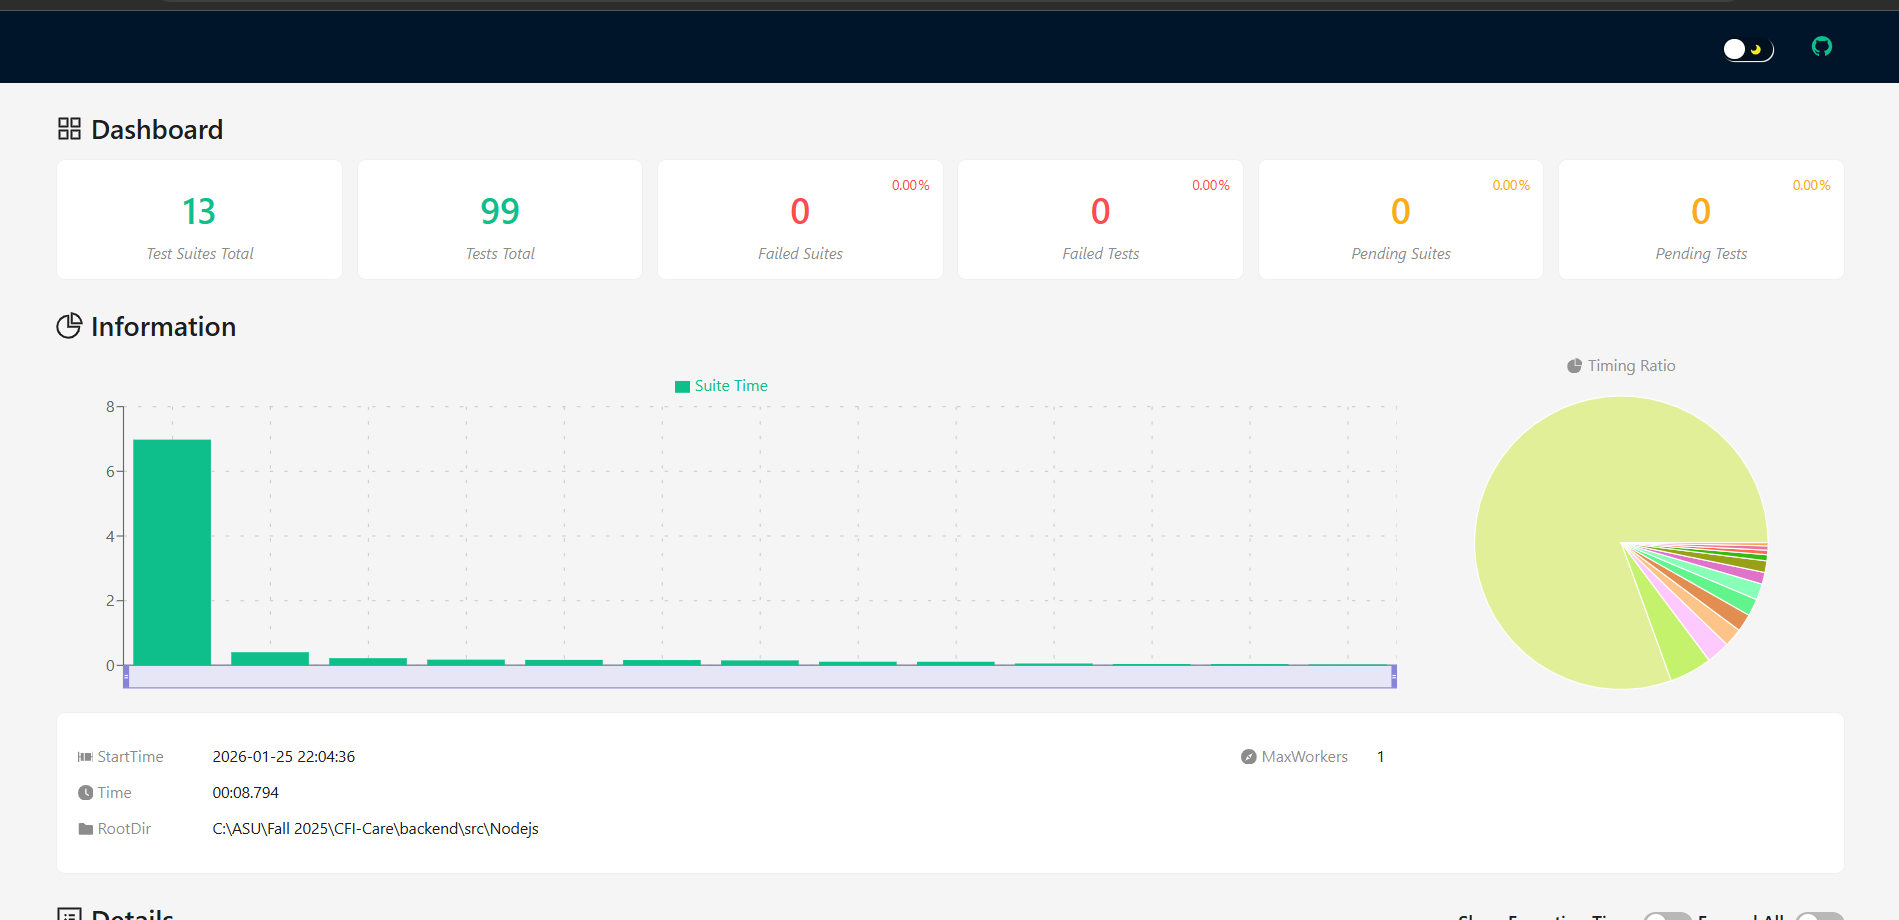
\includegraphics[width=0.8\textwidth]{Testing/Images/BackendTesting1.png}
    \caption{Unit and integration test suite results.}
    \label{fig:test-matrix-unit-integration}
\end{figure}

\begin{figure}[H]
    \centering
    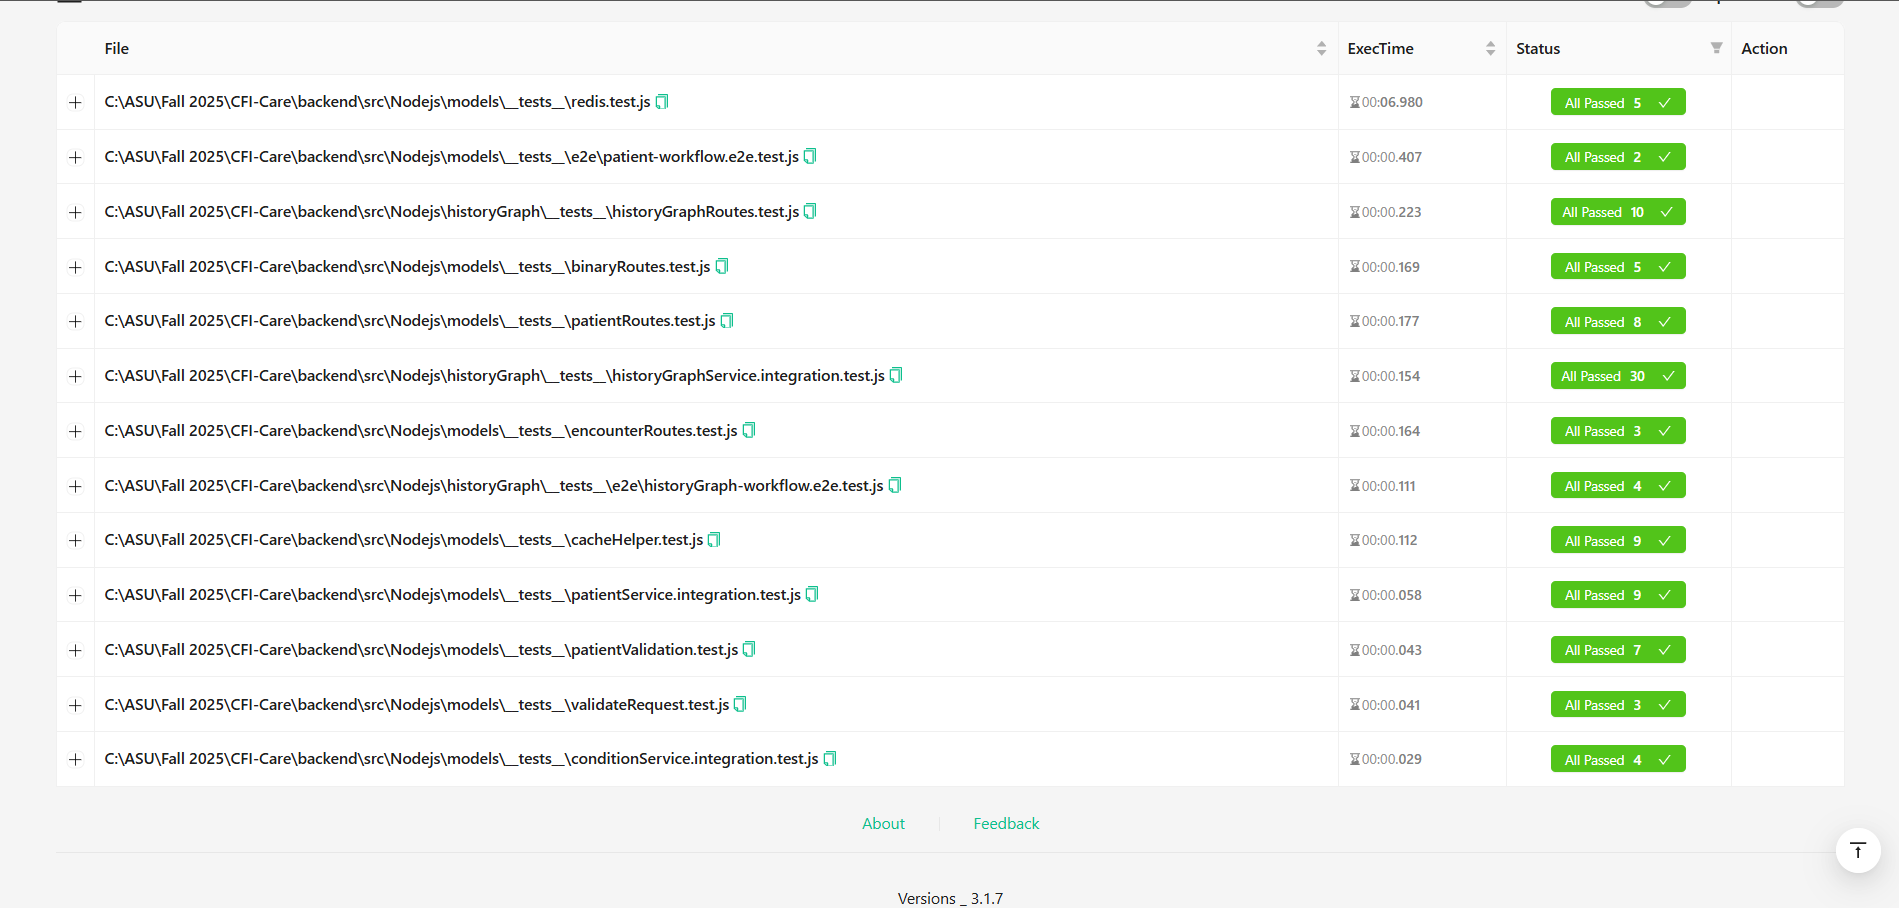
\includegraphics[width=0.8\textwidth]{Testing/Images/BackendTesting2.png}
    \caption{End-to-end and database workflow suite results.}
    \label{fig:test-matrix-e2e-db}
\end{figure}

\subsection{Interpretation of Results}

\begin{itemize}
  \item All 20 FHIR resource service unit tests pass, confirming that the
        cache-first read, write-triggered invalidation, and FHIR error-propagation
        paths are correct for every resource type exposed by the backend.
  \item The four route contract suites are green, indicating stable HTTP
        contracts at the controller layer for patients, encounters, binary
        resources, and the history graph API.
  \item Both e2e suites pass, including the eight history-graph scenarios that
        cover branch-state transitions, linker node auto-creation and removal,
        and concurrent multi-branch graphs.
  \item Live-environment checks for Redis and Postgres pass when the backing
        services are reachable; these are marked \textit{Pass*} (conditional)
        and excluded from the default CI target.
  \item The \texttt{historyGraphService.integration} suite now contains concrete
        assertions covering node/edge CRUD and branch-state persistence through
        the PostgreSQL mock, closing the gap noted in earlier development
        iterations.
\end{itemize}

\subsection{Gaps and Next Steps}

\begin{enumerate}
    \item Extend negative-path e2e coverage for encounter and condition endpoints,
          aligning status codes and error-body shapes with the route contract tests.
    \item Add contract tests to lock the TOON export and \texttt{\$everything}
          bundle payload shapes against accidental regression.
    \item Document and script external-service startup (Redis, Postgres, FHIR
          stub) to enable the full \texttt{test:all} target in CI without
          manual environment setup.
    \item Raise coverage thresholds incrementally toward 80\% as the history
          graph service integration suite matures.
\end{enumerate}
